\documentclass[number]{assignment}
\usepackage{titlepage}
\usepackage{ncolor}
\usepackage{math}
\usepackage{enumitem}
\usepackage{multicol}
\usepackage{float}
\usepackage{pdflscape}
\usepackage{tikz}

\setprimary{purple}

\name{Daniel}{Fitzmaurice}
\studentnumber{43961229}
\coursecode{deco2800}

\linespread{1.1}
\setlength{\columnseprule}{0.4pt}

\begin{document}
\begin{landscape}
\headfoot
\begin{multicols}{3}

% \heading{Team}
% Complementary Skills; Mutual Accountability; Common Commitment; Shared Goal; Collective Work Products; More than the sum of its parts\\
% \subheading{Meetings}
% Hogging -- talking too much; Flogging -- beating an issue to death; Frogging -- jumping from topic to topic; Bogging -- getting stuck on an issue; Ignoring the Elephant in the Corner\\

\heading{Software Architecture}
\subheading{Quality}
Cohesion -- Degree to which elements of a module fit together\\
Coupling -- Degree of interdependence between modules\\
% \begin{multicols}{2}
% 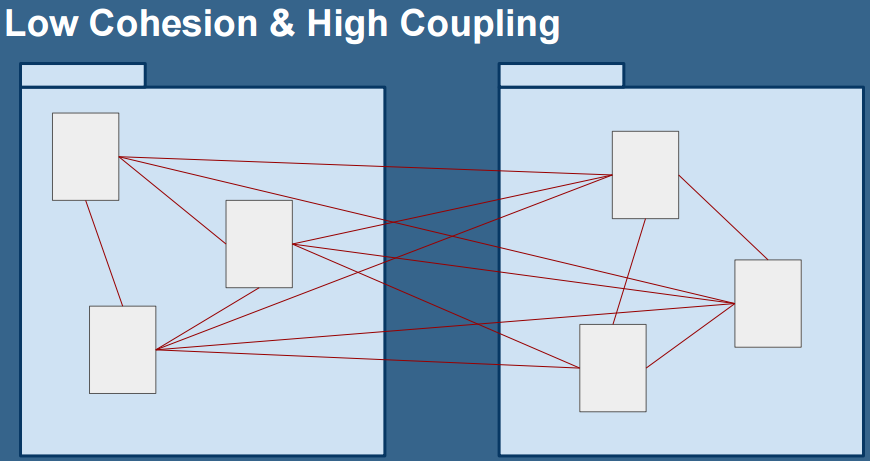
\includegraphics[width=\linewidth]{LowCHighC.png}
% 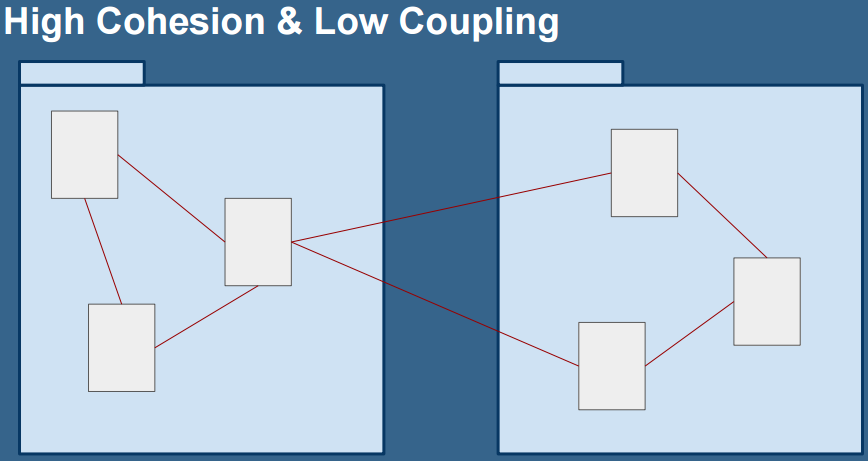
\includegraphics[width=\linewidth]{HighCLowC.png}
% \end{multicols}

\heading{Continuous Integration}
Merge Frequently; Don't push broken code; Don't push untested code; Don't push when the build is broken; If the build is broken, fix it\\

\heading{Test-Driven Development}
A software development methodology based on: Short development iterations, Satisfying pre-prepared test cases. An independent offshoot of Agile methodologies. Based on using automated unit testing to drive software development.
\subsubheading{How Many Tests?}
Test or both black-box and glass-box. As the programmer add glass-box tests for: Conditionals, Loops, Operations, Polymorphism.
\begin{multicols}{2}
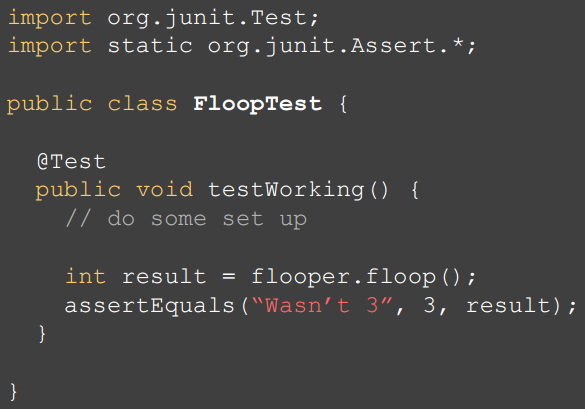
\includegraphics[width=\linewidth]{test1.png}
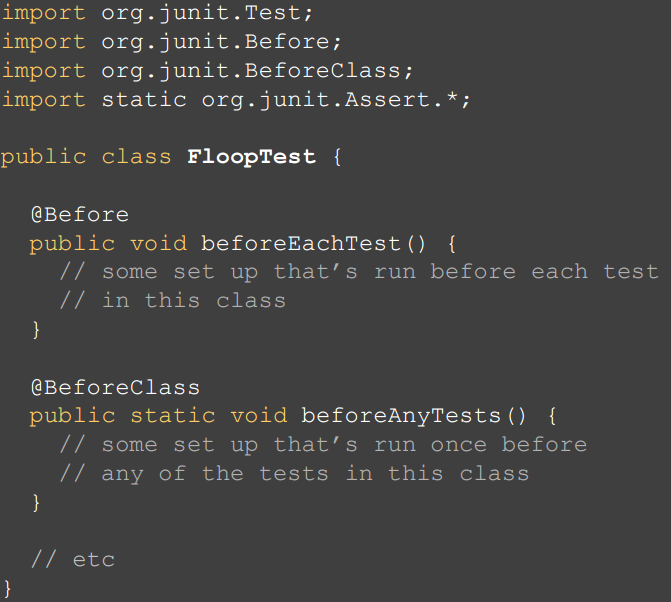
\includegraphics[width=\linewidth]{test2.png}
\end{multicols}
\subheading{Test-Driven Dev: Red, Green, Refactor}
\begin{multicols}{2}
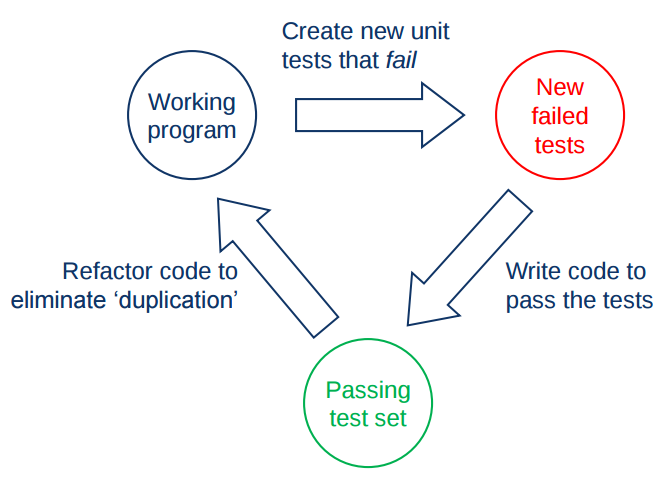
\includegraphics[width=\linewidth]{Cycle.png}
Applying Test-Driven Development relies on the existence of an automated unit testing environment. You are obliged to maintain a suite of test cases. Code must not be released until is has associated tests. The test are written \textbf{before} the code.
\end{multicols}
\subheading{Refactoring}
Code that needs refactoring has: Duplication, Unclear intent, Tight coupling, Pure data classes, Over-sized or under-sized classes, Complex or long methods, Switch statements instead of polymorphism.
\subheading{Mocking}
\textbf{\firstletter{D}ummies} - test objects which are never used but exist only to satisfy syntactic requirements\\
\textbf{\firstletter{S}tubs} - test objects whose methods return fixed values, and support the specific test cases only\\
\textbf{\firstletter{F}akes} - test objects whose methods work but have only limited functionality\\
\textbf{\firstletter{M}ocks} - test object which know how they're meant to be used, e.g. the sequence in which their methods should be called (allowing behavioural verification instead of just state verification)

\heading{Pair Programming}
Constant review from two people ensures fewer defects. Works well for mentoring: inexperienced staff, new team members, learning new techniques or tools.\\
\textbf{\firstletter{D}river} - person at the keyboard\\
\textbf{\firstletter{N}avigator} - focusing on design\\
Both need to be actively engaged - keep a running commentary\\
Switch roles frequently - every few minutes
\subheading{Ping-Pong Programming}
Driver writes a failing unit test. Driver \& Navigator switch roles. New driver implements code to pass test - then write a new failing unit test. Switch roles again

\heading{Class Model}
\subheading{Class Icon}
\begin{tabular}{|l|}
\hline
Employee \texttt{(Class Name)}\\\hline
-employeeNumber:String \texttt{(Attribute)}\\
-\underline{nextEmployeeNumber:String} \texttt{(Static Attribute)}\\
-qualification:Qualification[]\\\hline
+addQualification(qual:Qualification) \texttt{(Operation)}\\
+getDepartment():Department\\
+changeDepartment(dept:Department)\\\hline
\end{tabular}
\subheading{Association}
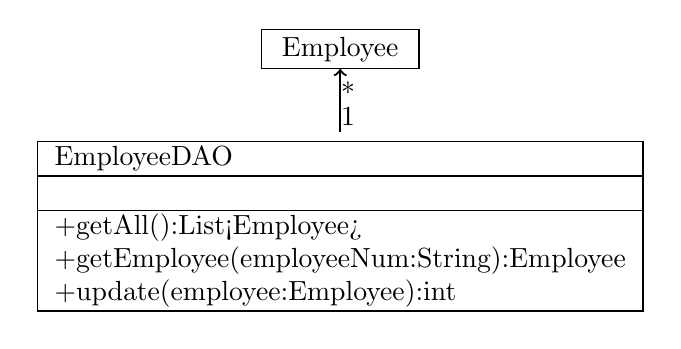
\begin{tikzpicture}[scale=1, transform shape]
\draw (-1,1) rectangle (1,1.5) node[pos=.5] {Employee};
\draw[thick,->] (0,.2) -- (0,1);
\draw (.1,.4) node {1};
\draw (.1,.7) node {*};
\draw (0,-1) node(t) {
    \begin{tabular}{|l|}
        \hline EmployeeDAO\\\hline\\
        \hline
        +getAll():List<Employee>\\
        +getEmployee(employeeNum:String):Employee\\
        +update(employee:Employee):int\\\hline
    \end{tabular}
};
\end{tikzpicture}
Navigability; arrow in direction of usage, no arrow is bi-directional. Multiplicity; min..max (or n), * is unlimited.
\subheading{Aggregation}
Strong relationship ``has a''. Hollow diamond
\subheading{Composition}
Strong relation ``is part of''. When composite is destroyed so is the part coincident life-span. Filled diamond
\subheading{Inheritance/Subtyping}
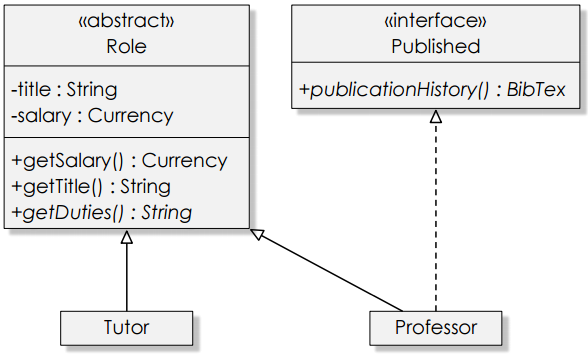
\includegraphics[width=\linewidth]{inheritance.png}
Generalisation/Specialisation: solid line, hollow arrow head. Implements: dashed line, hollow arrow head. Italics == abstract.
\subheading{Packages}
Dashed line = dependency. Solid line = Nesting

\heading{Design Patterns}
Apply at various levels of abstraction. Are not reusable classes. Are not complex, domain-specific designs. Are limited in scope. Capture design intent, but not the full detail.
\subheading{Common Language}
Provide a common language for describing solutions; Each window is a composite - with decorators providing titles and scroll bars, To save memory - each image is a flyweight.
\subheading{Pattern Form (GOF)}
Pattern Name - short descriptive moniker and any aliases. Intent - short statement summarizing what problem it solves. Motivation - scenario that describes a problem this pattern solves. Applicability - how to identify when to use this pattern. Structure - description of class relationships and the object interactions. Participants - classes making up the pattern and their responsibilities. Collaborations - how the classes collaborate to perform their responsibilities. Consequences - benefits and trade-offs of using the pattern. Implementation - hints for implementing the pattern (consider language specific issues). Known Uses - examples of the use of this pattern in real systems (the Rule of Three). Related Patterns.
\subheading{Common Patters}
\subsubheading{Singleton}
\textbf{Intent:} Ensure a class only has one instance, and provide a global point of access to it (\texttt{getInstance()} function)
\subsubheading{Observer}
\textbf{Intent:} Define a one-to-many dependency between objects so that when one object changes state, all its dependents are notified and updated automatically.\\
\textbf{Consequences:} Loose coupling between Subject and Observer, Broadcast communication.
\subsubheading{Composite}
\textbf{Intent:} Compose objects into tree structures to represent whole-part hierarchies. Composite lets clients treat individual objects and compositions of objects uniformly.\\
\textbf{Examples:} Menu Bars, Graphics.
\subsubheading{Command}
Encapsulate a request as an object, thereby letting you parameterize clients with different requests.
\subsubheading{Visitor}
Represent an operation to be performed on the elements of an object structure.
\subsubheading{State}
Allow an object to alter its behavior when its internal state changes.
\subsubheading{Lazy Loading}
Avoid creating a large/complex/expensive object until you actually need it. Create a placeholder object that can be substituted out when the real object is actually needed.\\
\textbf{Proxy} - loads real object when data is accessed then forwards messages to real object (delegates).\\
\textbf{Ghost} - real object is created but without any data. Loads data when a method is invoked.
\subsubheading{Radial Menus}
\textbf{Intent:} Present user commands or choices radiating out from a central point.\\
\textbf{Similar Patterns:} Icons instead of Text.\\
\textbf{Advantages:} Shorter average distance to each item, greater distance between each item, faster interaction for expert users, works well for selecting graphical options.\\
\textbf{Disadvantages:} Doesn't scale/nest as well as vertical menus (best for 3-12 items or so), not as intuitive to read for the novice user, less familiar, text has to remain horizontal.
\subheading{Anti-Patterns}
Some things look like patterns, but make things worse, not better. Knowing these is almost as valuable as knowing the ``good'' patterns.

\heading{Code Smells}
Code smells refer to any symtom in the source code that could possibly indicate a deeper problem. Code smells are not the problem. They do not produce compile errors and are not even bugs. Simply, they are evidence that there might be a bug or other issue nearby.
\subheading{Code Smells V Anti-Patterns}
Code smells are not the problem, however the benefit of understanding code smells is to help you discover and correct the anti-patterns and bugs that are the real problems.

\heading{User-Centered Design}
Understand -> Define -> Ideate(Sketch) -> Prototype -> Test -> Deliver!

\heading{Debuggin Process}
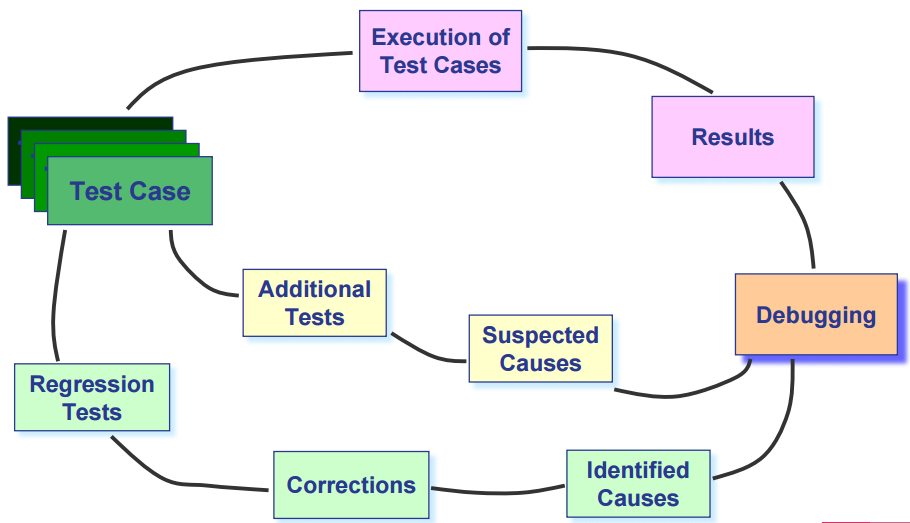
\includegraphics[width=\linewidth]{DebugProcess.png}

\heading{Logging}
\subheading{java.util.logging}
Levels: SEVERE, WARNING, INFO, CONFIG, FINE, FINER, FINEST (in order, also OFF and ALL). Level of the logger is a cutoff for recording messages
\subheading{Log4J}
Levels: FATAL, ERROR, WARN, INFO, DEBUG, TRACE (also OFF, ALL)
\subheading{slf4j}
Brings all the loggers together, enabling switching during runtime or on compilation. Avoids every library having its own logging facility. Uses all the log levels of log4j but FATAL.

\heading{System}
Jenkins -- Builds the changes to the repo; SonarQube -- checks for codesmells and code errors; Gradle -- For testing and running on local machine\\

\heading{JDBC(Java DataBase Connectivity)}
Standard library for relational databases. Standardises: Connecting, Queries and Updates, Results. Does not standardize SQL syntax (Sends strings).
\subheading{Drivers}
JDBC Driver Manager - Communicates with vendor-specific drivers that perform the real communication with the database.
\subheading{Plan for changes}
Limit data access to single area of code and don't distribute JDBC calls throughout the code. Don't return JDBC-specific objects from the data-access layer (Return ordinary Java Objects).
% \subheading{Basic Steps}
% \textbf{1.} Define the Connection URL\\
% \textbf{2.} Establish the Connection\\
% \textbf{3.} Create a Statement object\\
% \textbf{4.} Execute a query\\
% \textbf{5.} Process the results\\
% \textbf{6.} Close the connection\\

\heading{Apache Derby}
Written in Java. Good for small/medium applications (less than gig size, few queries/second). \textbf{Embedded mode:} Database runs in same VM as Java app. Does not accept network connections. Perfect for simple self-contained applications (easy setup). \textbf{Standalone mode:} Runs in seperate VM. Accepts network connections.

\heading{Prepared Statements}
Repeatedly executing query or update where format stays consistent, but values change.
\subheading{Advantages}
Move convenient than string concatenation. Much less susceptible to SQL injection attacks.

\heading{Advanced Features}
\subheading{Transactions}
By default, after each SQL statement is executed the changes are automatically committed to the database. Change with \texttt{connection.setAutoCommit(false);}
\subheading{More Features}
Stored procedures, Changing buffer size, Connection pooling, Hibernate/JPA and other ORM tools.

\heading{Flyway}
Store versions of database in metadata. Migrate from one version to the next using SQL or Java. Select database version in Gradle.

\heading{DBUnit}
Used for DataBase testing. Assumes there is a test database. Runs tests over the database.

\heading{JDBI}
Intermediate level relational database library. Methods map to single SQL statements.\\

\heading{JDBC v JDBI v JPA v JDO}
\textbf{JDBC:} Oriented towards database usage. \textbf{JDBI:} Oriented towards object usage. \textbf{JPA:} Focus on modelling. \textbf{JDO:} Focus on object modelling.

\end{multicols}
\end{landscape}
\end{document}